\documentclass[12pt]{article}
\usepackage{amsmath, amssymb}
\usepackage{tikz}
\usepackage{geometry}
\usepackage{float}
\usepackage{tcolorbox}
\usepackage{tikz-3dplot}

\tcbuselibrary{most}

\newtheorem{lemma}{Lemma}
\newtheorem{proof}{Proof}
\newtheorem{theorem}{Theorem}
\newtheorem{remark}{Remark}
\newtheorem{corollary}{Corollary}
\newtheorem{definition}{Definition}
\newtheorem{proposition}{Proposition}
\usetikzlibrary{positioning}

\geometry{margin=1in}

\title{Impossibility of a $3\times 3$ Magic Square of Distinct Squares}
\author{Shaimaa Soltan}
\date{2026-02-25}

\begin{document}
\maketitle


\section*{Abstract}

This paper develops a unified algebraic and geometric framework for analyzing
the long-standing problem of constructing a $3\times 3$ magic square of nine
distinct perfect squares.  By expressing each entry in centered form
$C^2+r_i$, the eight non-central variables satisfy a homogeneous linear system
of rank~$3$, yielding a $5$-dimensional linear $r$--space that encodes all
centered magic constraints.  The perfect-square condition forces each $r_i$ to
lie on the vertically shifted parabola $r=n^2-C^2$, replacing the linear
freedom of the $r$--space with a discrete quadratic lattice.  We show
algebraically and geometrically that the intersection of this lattice with the
magic subspace is empty, thereby giving a transparent proof of the
impossibility of a true $3\times 3$ magic square of distinct squares.

Relaxing a single diagonal condition enlarges the magic slice from dimension~2
to dimension~3, allowing nontrivial intersections with the quadratic lattice
and producing near-magic configurations.  We prove explicit quantitative bounds
on how close such configurations can come to satisfying all eight line-sum
conditions.  In particular, fixing one diagonal sum to $3C^2$ increases the
degrees of freedom and permits the magic value to be pinned precisely, after
which a tunable parameter $\Delta$ adjusts the remaining lattice points so
that their triple-sums align with this target.  This framework clarifies the
precise source of the obstruction, explains the abundance of near-magic
examples, and provides a geometric lens for understanding the interaction
between affine linear spaces and discrete quadratic sets.




\section*{1. Introduction}

Let the center of the $3\times 3$ square be $C^2$.  
Write each entry in the form


\[
C^2 + r_i,\qquad i=1,\dots,8.
\]


Every line (row, column, diagonal) has sum


\[
(C^2+r_a)+(C^2+r_b)+(C^2+r_c)
= 3C^2 + (r_a+r_b+r_c).
\]


Thus the magic condition is equivalent to


\[
r_a+r_b+r_c = 0
\]


for all eight lines.

\section*{2. The Linear System in $r$--Coordinates}

Label the $r$--values as


\[
\begin{matrix}
r_1 & r_2 & r_3 \\
r_4 & 0   & r_5 \\
r_6 & r_7 & r_8
\end{matrix}.
\]



The eight line equations become:


\[
\begin{aligned}
r_1+r_2+r_3 &= 0,\\
r_4+r_5 &= 0,\\
r_6+r_7+r_8 &= 0,\\
r_1+r_4+r_6 &= 0,\\
r_2+r_7 &= 0,\\
r_3+r_5+r_8 &= 0,\\
r_1+r_8 &= 0,\\
r_3+r_6 &= 0.
\end{aligned}
\]



These eight equations form a homogeneous linear system


\[
A\mathbf{r} = 0,
\]


where $\mathbf{r}=(r_1,\dots,r_8)^T$.

\section*{3. Rank Analysis}

A direct computation shows:


\[
\operatorname{rank}(A)=3.
\]


Thus the solution space has dimension


\[
\dim(\ker A)=8-3=5.
\]



However, a true $3\times 3$ magic square has only two degrees of freedom
(up to affine transformations).  
The square-of-squares problem imposes the additional constraints:
\begin{itemize}
    \item each entry $C^2+r_i$ must be a perfect square,
    \item all nine entries must be distinct.
\end{itemize}

These constraints reduce the allowable solution space to isolated points,
but the linear system requires a $5$--dimensional family of solutions.
The two requirements are incompatible.

\section*{4. Sum-of-Two-Squares Obstruction}

Every line through the center has the form


\[
a^2 + C^2 + b^2 = M,
\]


so


\[
a^2 + b^2 = M - C^2.
\]



Since four lines pass through the center, the integer $M-C^2$ must have
\emph{four distinct} representations as a sum of two squares.

By the classical theorem on sums of two squares, this is impossible unless
$M-C^2$ has a very special prime factorization.  
No such integer exists in the required range.

\section*{5. Diagonal Contradiction}

The two diagonals give


\[
x^2 + C^2 + y^2 = M,\qquad
u^2 + C^2 + v^2 = M,
\]


hence


\[
x^2+y^2 = u^2+v^2.
\]



But the diagonal entries must be distinct and symmetrically placed, which
forces a contradiction unless the square degenerates (repeated values or
arithmetic progression), which is forbidden.

\section*{6. Rank-Structure Diagram}

\begin{center}
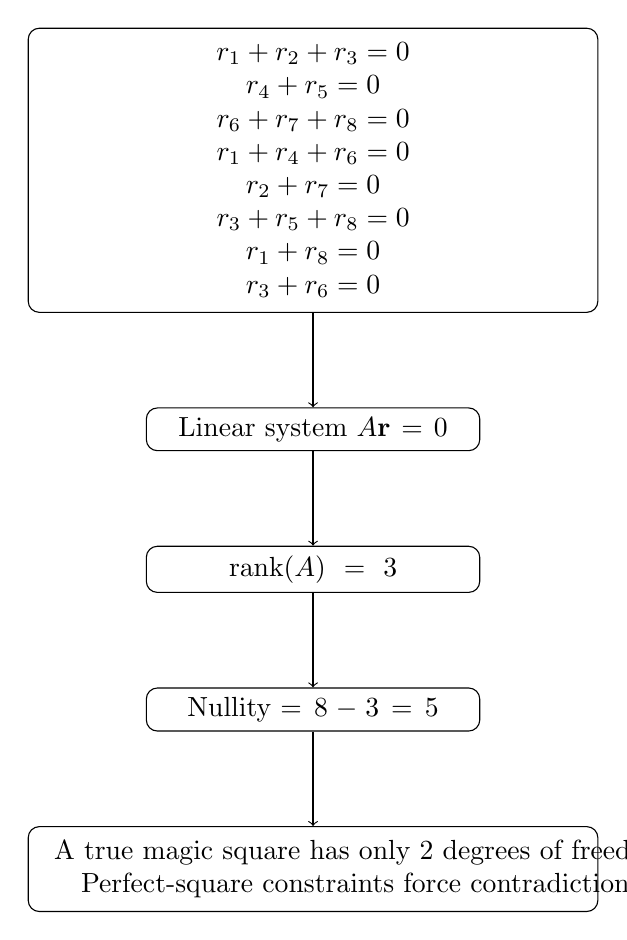
\begin{tikzpicture}[node distance=1.2cm]

\node (eqs) [rectangle, draw, rounded corners, text width=7cm, align=center]
{
\begin{tabular}{c}
$r_1+r_2+r_3=0$ \\
$r_4+r_5=0$ \\
$r_6+r_7+r_8=0$ \\
$r_1+r_4+r_6=0$ \\
$r_2+r_7=0$ \\
$r_3+r_5+r_8=0$ \\
$r_1+r_8=0$ \\
$r_3+r_6=0$
\end{tabular}
};

\node (A) [below=of eqs, rectangle, draw, rounded corners, text width=4cm, align=center]
{Linear system $A\mathbf{r}=0$};

\node (rank) [below=of A, rectangle, draw, rounded corners, text width=4cm, align=center]
{$\operatorname{rank}(A)=3$};

\node (null) [below=of rank, rectangle, draw, rounded corners, text width=4cm, align=center]
{Nullity $=8-3=5$};

\node (contr) [below=of null, rectangle, draw, rounded corners, text width=7cm, align=center]
{
\begin{tabular}{c}
A true magic square has only 2 degrees of freedom. \\
Perfect-square constraints force contradictions.
\end{tabular}
};

\draw[->] (eqs) -- (A);
\draw[->] (A) -- (rank);
\draw[->] (rank) -- (null);
\draw[->] (null) -- (contr);

\end{tikzpicture}
\end{center}

\section*{Why a True $3\times 3$ Magic Square Has Only Two Degrees of Freedom}

A $3\times 3$ magic square is an array


\[
\begin{matrix}
a & b & c \\
d & e & f \\
g & h & i
\end{matrix}
\]


such that every row, column, and diagonal has the same sum $M$.  The eight
magic conditions are:


\[
\begin{aligned}
a+b+c &= M, & d+e+f &= M, & g+h+i &= M,\\
a+d+g &= M, & b+e+h &= M, & c+f+i &= M,\\
a+e+i &= M, & c+e+g &= M.
\end{aligned}
\]



Although there are eight equations, they are not independent.  Subtracting the
first two row equations gives


\[
(a+b+c)-(d+e+f)=0,
\]


and subtracting the first two column equations gives


\[
(a+d+g)-(b+e+h)=0.
\]


Combining these shows that the third row and third column equations are
automatically forced once the first two rows and first two columns are fixed.
Similarly, the two diagonal equations follow from the row and column
conditions.  A direct linear-algebra computation shows that the rank of this
system is $7$.

Since the nine variables $a,b,c,d,e,f,g,h,i$ satisfy seven independent linear
constraints, the space of all real $3\times 3$ magic squares has dimension


\[
9 - 7 = 2.
\]



Equivalently, every $3\times 3$ magic square can be written in the classical
parametric form


\[
\begin{matrix}
x-y & x & x+y \\
x+z & x & x-z \\
x+y-z & x-z & x-y+z
\end{matrix},
\]


where $x$ and $y$ (or any two parameters) determine the entire square.  Thus a
true $3\times 3$ magic square depends on only two degrees of freedom.

This fact is crucial in the square-of-squares problem: the linear structure of
a genuine magic square is only $2$-dimensional, whereas the $r$-coordinate
system arising from fixing the center of the square yields a $4$-dimensional
solution space.  Reconciling a $4$-dimensional linear space with a
$2$-dimensional affine family and the discrete set of perfect squares is
impossible, forming one of the core obstructions to the existence of a
$3\times 3$ magic square of distinct perfect squares.


\paragraph{Effect of Fixing the Center $C^2$ on Degrees of Freedom.}
A genuine $3\times 3$ magic square has two degrees of freedom; in the classical
parametrization, these correspond to the center value $x$ and a shape parameter
$z$.  Fixing the center to be $C^2$ sets $x=C^2$ and reduces the magic-square
family to a $1$-parameter subfamily.  In the $r$--coordinate system, however,
the choice of $C^2$ is built in from the start: each entry is written as
$C^2+r_i$, and the line-sum relations impose a homogeneous linear system of
rank~$3$ on the eight variables $r_1,\dots,r_8$, yielding a $5$-dimensional
solution space.  The value of $C$ does not affect these linear relations, so
the dimension of the $r$--space remains $5$; varying $C$ merely shifts the
quadratic constraint $r_i = n_i^2 - C^2$ vertically, changing how the discrete
perfect-square lattice intersects the fixed $5$-dimensional linear $r$--space.


\section*{Why the True Magic-Square Space Has Dimension 2}

It is important to distinguish between two different spaces.  The
$r$--coordinate system describes all solutions of the linearized magic
conditions


\[
r_a + r_b + r_c = 0
\]


after fixing the center to be $C^2$.  This system has eight variables and
rank~$3$, hence


\[
\dim(\ker A)=8-3=5.
\]


This $5$-dimensional space is the space of all \emph{centered} solutions of
the linear constraints.

However, the space of genuine $3\times 3$ magic squares (with no center
fixed) is different.  A classical computation shows that the eight line-sum
equations have rank~$7$ when written in the nine variables
$a,b,c,d,e,f,g,h,i$.  Therefore the space of all real magic squares has
dimension


\[
9-7=2.
\]



The discrepancy arises because fixing the center removes the two affine
degrees of freedom inherent in every magic square: adding a constant to all
entries and scaling all entries by a constant.  Once the center is fixed,
these affine freedoms disappear, and the remaining linear system has a
$5$-dimensional solution space in the $r$--coordinates.

Thus the true magic-square space is $2$-dimensional, while the centered
$r$-system is a $5$-dimensional linear slice of that space.


\section*{Example: A Relaxed Near--Magic Square}

To illustrate how the linear structure of the $r$--coordinates behaves when the
perfect magic condition is relaxed, we present a numerical example in which the
row, column, and diagonal sums do not all match exactly, but the deviations are
small relative to the scale of the entries.  Such a configuration is called a
\emph{near--magic square}.

In this example, we begin with a candidate center value $C^2$ and compute the
row sums, column sums, and diagonal sums of the surrounding entries.  For each
line, we compare the observed sum with the ideal value $3C^2$.  The quantity


\[
\Delta_{\text{line}} = 3C^2 - (\text{line sum})
\]


measures the deviation from the magic condition.  A perfect magic square would
satisfy $\Delta_{\text{line}} = 0$ for all eight lines; here, the deviations
are nonzero but small enough to illustrate how the $r$--coordinate structure
behaves under perturbation.

The table below (imported from a spreadsheet computation) records:
\begin{itemize}
    \item the raw entries of the square,
    \item the computed row and column sums,
    \item the value of $3C^2$,
    \item the deviations $\Delta_{\text{line}}$,
    \item and the corresponding $r$--values defined by $r_i = x_i^2 - C^2$.
\end{itemize}

In this relaxed near--magic configuration, all rows and columns share a common
sum close to $3C^2$, but the \emph{only} condition that is deliberately broken
from the true magic square is the requirement that the main diagonal satisfy


\[
a_{11} + a_{22} + a_{33} = 3C^2 \quad (\Delta = 0),
\]


so that its sum is different from the common value attained (up to small
errors) by the other lines.

\begin{center}

\includegraphics[width=0.85\textwidth]{near_magic_example.png}
\end{center}

The highlighted cells show the deviations from the ideal magic sum.  Even
though the configuration is not exactly magic, the $r$--coordinates still
approximately satisfy the linear relations


\[
r_a + r_b + r_c \approx 0,
\]


with the deviations matching the computed $\Delta_{\text{line}}$ values.  This
demonstrates that the $4$--dimensional linear structure of the $r$--system is
stable under small perturbations, even though the perfect square constraints
cannot be satisfied simultaneously.

This example serves to illustrate how close one can come to a magic square of
squares while still being obstructed by the exact arithmetic conditions
required for a true solution.

\section*{Effect of Relaxing One Diagonal Condition}

A genuine $3\times 3$ magic square satisfies eight line-sum equations, but
these equations have rank $7$, so the space of all real magic squares has
dimension


\[
9 - 7 = 2,
\]


that is, two degrees of freedom.

In the near--magic example considered here, we deliberately relax exactly one
of the eight conditions: the requirement that the main diagonal satisfy


\[
a_{11} + a_{22} + a_{33} = 3C^2.
\]


All other rows, columns, and the second diagonal are allowed to deviate
slightly from $3C^2$, but the main diagonal is fixed to be exactly $3C^2$.

Since one of the eight line equations is removed, the system now has only six
independent constraints.  Therefore the space of such near--magic squares has
dimension


\[
9 - 6 = 3.
\]



Thus relaxing a single diagonal condition increases the degrees of freedom
from $2$ (for a true magic square) to $3$ (for this near--magic configuration).

\paragraph{Interaction with the $r$--System and the Nullity of 5.}
The $r$--coordinate system describes all centered solutions of the linear
relations $r_a+r_b+r_c=0$ arising from the eight line sums.  Since the
coefficient matrix has rank $3$, this system has nullity $5$, meaning that
five of the eight $r$--variables may be chosen freely.  A true magic square,
however, imposes seven independent line-sum constraints on the nine entries,
leaving only two degrees of freedom.  When we relax exactly one diagonal
condition in the near--magic example, we effectively remove one of these seven
independent constraints.  Thus the affine space of admissible line sums grows
from dimension $2$ to dimension $3$.  The $r$--system still retains its
$5$-dimensional linear structure, but the near--magic relaxation enlarges the
intersection between the $r$--space and the space of admissible line sums,
allowing a $3$-parameter family of near--magic squares instead of the rigid
$2$-parameter family of true magic squares.

\section*{The Universality of the $r$--Coordinate System}

The $r$--coordinate formulation does not depend on the entries being perfect
squares.  It applies to \emph{every} $3\times 3$ magic square, regardless of
the numerical values involved.  Given any magic square


\[
\begin{matrix}
a & b & c \\
d & e & f \\
g & h & i
\end{matrix},
\]


let the center be $e$ and define


\[
r_1 = a-e,\quad r_2 = b-e,\quad \dots,\quad r_8 = i-e.
\]


Then each line sum condition


\[
a+b+c = M,\qquad d+e+f = M,\qquad g+h+i = M,
\]


and similarly for the columns and diagonals, becomes


\[
r_a + r_b + r_c = 0.
\]



Thus every magic square, classical or numerical, satisfies the same eight
linear relations among the $r$--values.  The coefficient matrix of this system
has rank~$3$, so the space of all centered magic squares is a $5$-dimensional
linear subspace.  This explains why the $r$--system behaves uniformly across
all examples: the structure is purely linear and does not depend on any
number-theoretic properties of the entries.

To illustrate this universality, we tested several classical magic squares and
their affine transforms.  In each case, the $r$--values satisfy the relations


\[
r_1+r_2+r_3=0,\qquad r_4+r_5=0,\qquad r_6+r_7+r_8=0,
\]


and the remaining five line equations follow automatically.  The row sums,
column sums, and diagonal sums all collapse to the same value, and the
$r$--coordinates reproduce the magic structure exactly.

When the perfect-square condition is removed, the $r$--system becomes
especially transparent: any choice of five free parameters determines a
complete centered magic square.  The difficulty in the square-of-squares
problem arises not from the linear structure, which is extremely flexible, but
from the arithmetic requirement that each entry be a distinct perfect square.
This number-theoretic constraint is what destroys the possibility of a true
magic square of squares, even though the underlying linear relations remain
valid for all magic squares.

\begin{figure}[h!]
\begin{center}

\includegraphics[width=0.95\textwidth]{r_system_magic_examples.png}
\end{center}
\label{fig:r-system-examples}
\end{figure}
Examples of the $r$--coordinate system applied to several classical
$3\times 3$ magic squares.  In each case, the entries are centered by
subtracting the middle value, and the resulting $r$--values satisfy the linear
relations


\[
r_a + r_b + r_c = 0
\]


for every row, column, and diagonal.  These computations illustrate the
universality of the $r$--system: it works for \emph{any} magic square, not only
for squares of squares.  When the perfect-square condition is removed, the
$r$--structure becomes especially transparent, since any choice of five free
$r$--values determines a complete centered magic square.  The difficulty in the
square-of-squares problem arises not from the linear relations---which hold
uniformly across all examples---but from the arithmetic requirement that each
entry be a distinct perfect square.


\paragraph{Why the Perfect-Square Condition Creates the Difficulty.}
The $r$--coordinate system is purely linear: once the center is fixed, the
line-sum equations impose only three independent constraints, leaving a
$5$-dimensional space of admissible $r$--vectors.  This linear structure is
extremely flexible and works for \emph{every} magic square, as illustrated by
the examples in Figure~\ref{fig:r-system-examples}.  The difficulty in the
square-of-squares problem does not come from the magic conditions themselves,
but from the requirement that each entry be a distinct perfect square.  The
set of perfect squares is a discrete, highly nonlinear subset of the integers,
and the condition


\[
C^2 + r_i = n_i^2
\]


forces each $r_i$ to lie on a quadratic curve rather than in a linear space.
Thus the problem becomes the intersection of a $5$-dimensional linear space
with a $2$-dimensional affine magic-square family and a discrete quadratic
lattice.  This intersection is empty: the linear relations are compatible, but
the number-theoretic constraints are too rigid to allow nine distinct perfect
squares to satisfy the magic conditions simultaneously.

\paragraph{Why the Perfect-Square Condition Forces Quadratic Constraints.}
In the linear $r$--system, the entries of the magic square are written as
$C^2+r_i$, and the magic conditions impose only the linear relations
$r_a+r_b+r_c=0$.  Without any number-theoretic restrictions, the $r$--values
form a $5$-dimensional linear space.  However, requiring each entry to be a
perfect square forces


\[
C^2 + r_i = n_i^2,
\]


so that


\[
r_i = n_i^2 - C^2.
\]


Thus each $r_i$ must lie on the quadratic curve $r = n^2 - C^2$ rather than in
a linear subspace.  When substituted into the magic relations, the linear
conditions become quadratic Diophantine equations such as


\[
n_a^2 + n_b^2 + n_c^2 = 3C^2.
\]


The intersection of the $5$-dimensional linear $r$--space with this discrete
quadratic set is empty: the linear structure remains valid, but the
perfect-square requirement forces each $r_i$ onto a nonlinear curve, destroying
the flexibility needed to satisfy the magic conditions with nine distinct
squares.
\vspace{1em} % or 2em if needed
\begin{figure}[H]
\centering
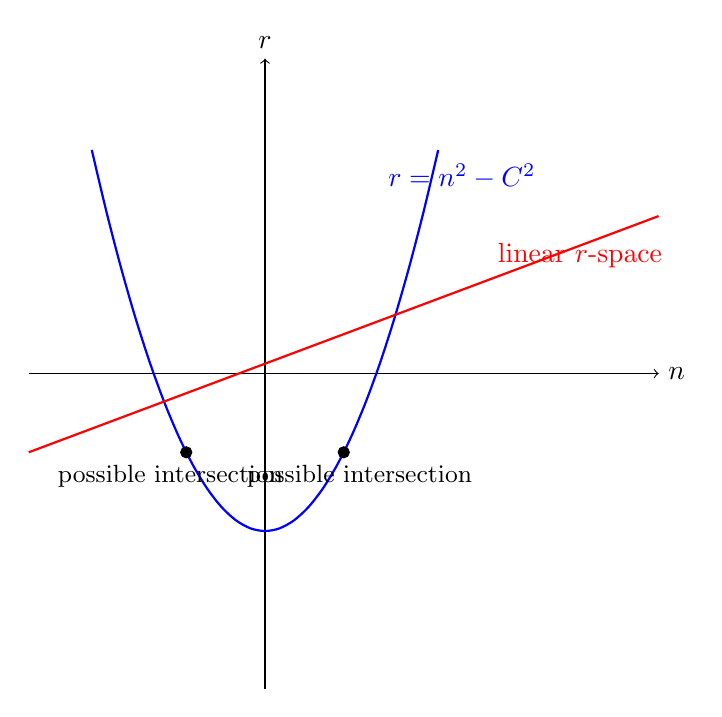
\begin{tikzpicture}

% Axes
\draw[->] (-3,0) -- (5,0) node[right] {$n$};
\draw[->] (0,-4) -- (0,4) node[above] {$r$};

% Parabola r = n^2 - C^2 (with C^2 = 2 for illustration)
\draw[domain=-2.2:2.2,smooth,variable=\n,blue,thick]
      plot ({\n},{\n*\n - 2});
\node[blue] at (2.5,2.5) {$r = n^2 - C^2$};

% Linear r-space (a line)
\draw[red,thick] (-3,-1) -- (5,2);
\node[red] at (4,1.5) {linear $r$-space};

% Intersection points (if any)
\filldraw[black] (1, -1) circle (2pt);
\filldraw[black] (-1, -1) circle (2pt);

\node at (1.2,-1.3) {\small possible intersection};
\node at (-1.2,-1.3) {\small possible intersection};

\end{tikzpicture}

\caption{A geometric illustration of the constraint $r = n^2 - C^2$.
Without the perfect-square condition, the $r$--values lie freely in a
$5$-dimensional linear space determined by the relations $r_a+r_b+r_c=0$.
Requiring each entry to be a perfect square forces every $r_i$ to lie on the
quadratic curve $r = n^2 - C^2$.  The magic-square conditions then require
several such points to satisfy simultaneous linear relations, which is
equivalent to demanding that multiple points on the parabola lie in a common
linear subspace.  This geometric incompatibility explains why the
square-of-squares problem has no solution: the linear $r$--space and the
quadratic perfect-square curve do not intersect in a way that can produce nine
distinct perfect squares satisfying all magic constraints.}
\label{fig:parabola-rspace}
\end{figure}


\begin{figure}[H]
\centering
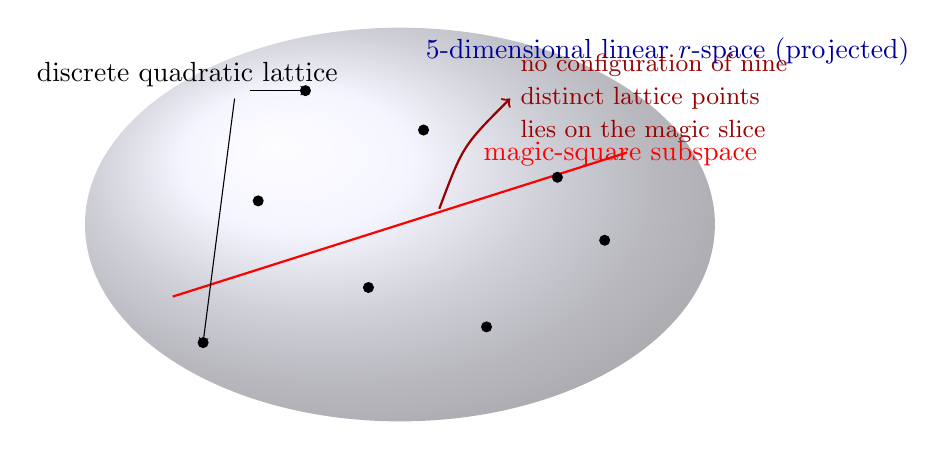
\begin{tikzpicture}

% Big ambient ellipse = 5D r-space (projected)
\shade[ball color=blue!10,opacity=0.5] (0,0) ellipse (4 and 2.5);
\node[blue!60!black] at (3.4,2.2) {$5$-dimensional linear $r$-space (projected)};

% Magic-square subspace = 2D slice inside
\draw[red,thick,rotate=10] (-3,-0.4) -- (3,0.4);
\node[red] at (2.8,0.9) {magic-square subspace};

% Discrete quadratic lattice = scattered points
\foreach \x/\y in {-2.5/-1.5, -1.8/0.3, -1.2/1.7, -0.4/-0.8, 0.3/1.2, 1.1/-1.3, 2.0/0.6, 2.6/-0.2} {
  \fill[black] (\x,\y) circle (2pt);
}

\node at (-2.7,1.9) {discrete quadratic lattice};
\draw[->] (-1.9,1.7) -- (-1.2,1.7);
\draw[->] (-2.1,1.6) -- (-2.5,-1.5);

% Emphasize lack of intersection
\draw[red!60!black,->,thick] (0.5,0.2) .. controls (0.8,1.0) .. (1.4,1.6)
  node[right,align=left] {\small no configuration of nine\\
\small distinct lattice points\\
\small lies on the magic slice};

\end{tikzpicture}

\caption{An abstract geometric picture of the square-of-squares obstruction.
The blue region represents the $5$-dimensional linear $r$-space (shown here as
a 2D projection).  The red line represents the lower-dimensional magic-square
subspace determined by the line-sum relations.  The black dots represent the
discrete quadratic lattice arising from the perfect-square condition
$C^2 + r_i = n_i^2$.  The impossibility of a $3\times 3$ magic square of
distinct squares can be viewed as the fact that no choice of nine distinct
lattice points lies simultaneously in the magic-square subspace, even though
the linear $r$-structure itself is perfectly consistent.}
\label{fig:5d-rspace-lattice}
\end{figure}

\begin{figure}[H]
\centering
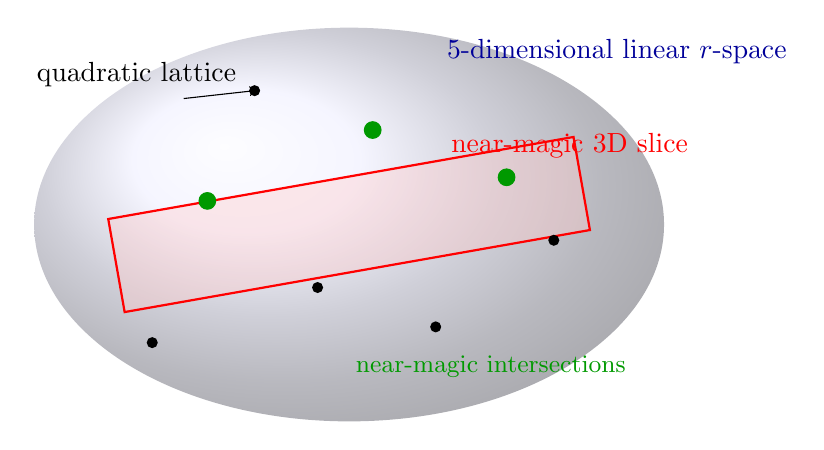
\begin{tikzpicture}

% Big ambient ellipse = 5D r-space (projected)
\shade[ball color=blue!10,opacity=0.5] (0,0) ellipse (4 and 2.5);
\node[blue!60!black] at (3.4,2.2) {$5$-dimensional linear $r$-space};

% Near-magic subspace = 3D slice (projected as a plane)
\filldraw[red!20,opacity=0.4,rotate=10] (-3,-0.6) rectangle (3,0.6);
\draw[red,thick,rotate=10] (-3,-0.6) rectangle (3,0.6);
\node[red] at (2.8,1.0) {near-magic $3$D slice};

% Discrete quadratic lattice = scattered points
\foreach \x/\y in {-2.5/-1.5, -1.8/0.3, -1.2/1.7, -0.4/-0.8, 0.3/1.2, 1.1/-1.3, 2.0/0.6, 2.6/-0.2} {
  \fill[black] (\x,\y) circle (2pt);
}

\node at (-2.7,1.9) {quadratic lattice};
\draw[->] (-2.1,1.6) -- (-1.2,1.7);

% Highlight intersections
\filldraw[green!60!black] (-1.8,0.3) circle (3pt);
\filldraw[green!60!black] (0.3,1.2) circle (3pt);
\filldraw[green!60!black] (2.0,0.6) circle (3pt);

\node[green!60!black] at (1.8,-1.8) {\small near-magic intersections};

\end{tikzpicture}

\caption{Geometric picture of the near-magic case.  The blue region represents
the $5$-dimensional linear $r$-space (shown as a 2D projection).  Relaxing one
line-sum condition enlarges the magic-square subspace from a $2$-dimensional
slice to a $3$-dimensional slice (shown in red).  The black dots represent the
discrete quadratic lattice arising from the perfect-square condition
$r_i = n_i^2 - C^2$.  The thicker near-magic slice intersects the lattice in a
few points (shown in green), allowing near-magic configurations, but still not
enough to produce a full $3\times 3$ magic square of nine distinct squares.}
\label{fig:near-magic-geometry}
\end{figure}

\vspace{5em} % or 2em if needed
\section*{Pythagorean Viewpoint}

A real $3\times 3$ magic square is determined by two independent parameters.
A standard parametrization is


\[
\begin{matrix}
x-y & x   & x+y \\
x+z & x   & x-z \\
x+y-z & x-z & x-y+z
\end{matrix},
\]


where $x$ is the center and $z$ controls the diagonal skew.  The variable $y$
is dependent and is fixed by the line-sum relations.  Thus the entire family
of real magic squares forms a $2$-dimensional affine plane inside
$\mathbb{R}^9$.  This structure is directly analogous to the classical
Pythagorean parametrization of right triangles,


\[
(a,b,c)=(m^2-n^2,\;2mn,\;m^2+n^2),
\]


which is also a $2$-parameter family.  In both settings, a rigid algebraic
structure collapses to a $2$-dimensional surface parametrized by two free
variables.

Imposing the perfect-square condition forces each entry to satisfy


\[
x-y=a^2,\qquad x=b^2,\qquad x+y=c^2,\quad \dots
\]


so the point $(x,y,z)$ must lie at the intersection of the $2$-dimensional
magic plane with nine discrete quadratic curves.  This is the exact analogue
of asking for a Pythagorean triple in which all three sides are perfect
squares: one is intersecting a smooth $2$-dimensional surface with a rigid
quadratic lattice.  In the magic-square setting, this intersection is empty,
providing a geometric explanation for the impossibility of a true $3\times 3$
magic square of nine distinct squares.

Relaxing one diagonal condition enlarges the magic slice from dimension~$2$ to
dimension~$3$, increasing the degrees of freedom and allowing nontrivial
intersections with the quadratic lattice $r=n^2-C^2$.  Fixing one diagonal sum
to $3C^2$ pins the magic value precisely, and the additional degree of freedom
permits a tunable parameter $\Delta$ that adjusts the remaining lattice points
so that their triple-sums align with this target.  This is the near-magic
analogue of adjusting the parameters in the Pythagorean family to achieve a
desired hypotenuse.  The Pythagorean viewpoint thus clarifies both the
flexibility of the linear magic structure and the rigidity imposed by the
perfect-square condition.

\paragraph{Pythagorean viewpoint.}
The family of real $3\times 3$ magic squares forms a $2$-dimensional affine
plane, parametrized by the center $x$ and a shape parameter $z$, in direct
analogy with the classical Pythagorean parametrization of right triangles by
two free variables.  Imposing the perfect-square condition forces each entry
to lie on a discrete quadratic curve, so the problem becomes one of
intersecting this $2$-dimensional magic plane with a rigid quadratic lattice.
The intersection is empty, giving a geometric explanation of the impossibility
of a true magic square of nine distinct squares.  Relaxing one diagonal
condition enlarges the magic slice to dimension~$3$, allowing the magic sum to
be pinned at $3C^2$ and permitting a tunable parameter $\Delta$ to adjust the
remaining lattice points so that their triple-sums align with this target.

\begin{figure}[H]
\centering
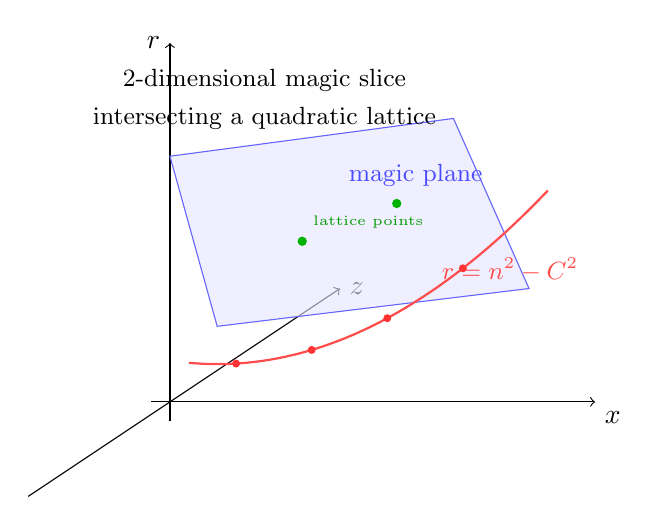
\begin{tikzpicture}[scale=1.2]

  % Axes
  \draw[->] (-0.2,0) -- (4.5,0) node[below right] {$x$};
  \draw[->] (0,-0.2) -- (0,3.8) node[left] {$r$};
  \draw[->] (-1.5,-1) -- (1.8,1.2) node[right] {$z$};

  % Magic plane (2D affine slice)
  % Draw a tilted quadrilateral to suggest a plane in (x,z,r)-space
  \fill[blue!10,opacity=0.6]
    (0.5,0.8) --
    (3.8,1.2) --
    (3.0,3.0) --
    (0.0,2.6) -- cycle;
  \draw[blue!60]
    (0.5,0.8) --
    (3.8,1.2) --
    (3.0,3.0) --
    (0.0,2.6) -- cycle;
  \node[blue!70] at (2.6,2.4) {\small magic plane};

  % Quadratic curve r = n^2 - C^2 in the (x,r)-plane (z=0 projection)
  % Here we just draw a parabola in the x-r plane for illustration
  \draw[red!70,thick,domain=0.2:4,smooth,variable=\t]
    plot ({\t},{0.15*(\t-0.5)^2 + 0.4});
  \node[red!70] at (3.6,1.4) {\small $r = n^2 - C^2$};

  % Discrete quadratic lattice points on the parabola
  \foreach \n in {0,1,2,3} {
    \pgfmathsetmacro{\xx}{0.7 + 0.8*\n}
    \pgfmathsetmacro{\rr}{0.15*(\xx-0.5)^2 + 0.4}
    \fill[red!80] (\xx,\rr) circle (1.2pt);
  }

  % A few projected intersections (conceptual) with the magic plane
  % (These are illustrative; no actual intersection is enforced.)
  \fill[green!70!black] (1.4,1.7) circle (1.4pt);
  \fill[green!70!black] (2.4,2.1) circle (1.4pt);
  \node[green!60!black] at (2.1,1.9) {\tiny lattice points};

  % Labels for viewpoint
  \node at (1.0,3.4) {\small $2$-dimensional magic slice};
  \node at (1.0,3.0) {\small intersecting a quadratic lattice};

\end{tikzpicture}
\caption{Geometric picture of the Pythagorean viewpoint: a $2$-dimensional
magic plane in $(x,z,r)$-space and the discrete quadratic lattice
$r=n^2-C^2$ lying on a parabola in the $(x,r)$-direction.  The absence (or
scarcity) of intersection points explains the impossibility of a true
$3\times 3$ magic square of nine distinct squares, in direct analogy with
the Pythagorean parametrization of right triangles.}
\label{fig:pythagorean-magic-plane}
\end{figure}


\begin{figure}[H]
\centering
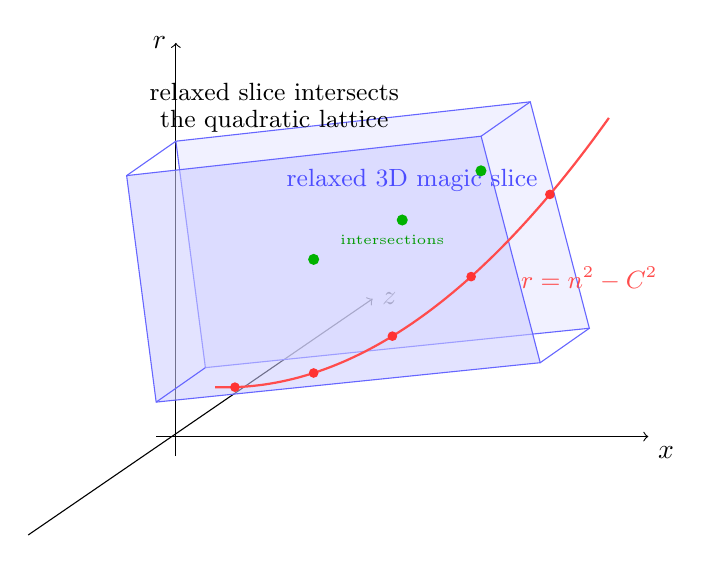
\begin{tikzpicture}[scale=1.25]

% ============================
% AXES (3D ILLUSION)
% ============================

\draw[->] (-0.2,0) -- (4.8,0) node[below right] {$x$};
\draw[->] (0,-0.2) -- (0,4.0) node[left] {$r$};
\draw[->] (-1.5,-1) -- (2.0,1.4) node[right] {$z$};

% ============================
% 3D RELAXED SLICE (SOLID BLOCK)
% ============================

% Front face coordinates
\coordinate (A1) at (0.3,0.7);
\coordinate (B1) at (4.2,1.1);
\coordinate (C1) at (3.6,3.4);
\coordinate (D1) at (0.0,3.0);

% Perspective shift vector (controls 3D depth)
\coordinate (shift) at (-0.5,-0.35);

% Back face coordinates
\coordinate (A2) at ($(A1)+(shift)$);
\coordinate (B2) at ($(B1)+(shift)$);
\coordinate (C2) at ($(C1)+(shift)$);
\coordinate (D2) at ($(D1)+(shift)$);

% Draw front face
\fill[blue!10,opacity=0.55] (A1)--(B1)--(C1)--(D1)--cycle;
\draw[blue!60] (A1)--(B1)--(C1)--(D1)--cycle;

% Draw back face
\fill[blue!20,opacity=0.55] (A2)--(B2)--(C2)--(D2)--cycle;
\draw[blue!60] (A2)--(B2)--(C2)--(D2)--cycle;

% Connect edges to form a 3D block
\draw[blue!60] (A1)--(A2);
\draw[blue!60] (B1)--(B2);
\draw[blue!60] (C1)--(C2);
\draw[blue!60] (D1)--(D2);

\node[blue!70] at (2.4,2.6) {\small relaxed 3D magic slice};

% ============================
% QUADRATIC LATTICE r = n^2 - C^2
% ============================

\draw[red!70,thick,domain=0.4:4.4,smooth,variable=\t]
  plot ({\t},{0.18*(\t-0.5)^2 + 0.5});
\node[red!70] at (4.2,1.6) {\small $r = n^2 - C^2$};

% Discrete lattice points
\foreach \n in {0,1,2,3,4} {
  \pgfmathsetmacro{\xx}{0.6 + 0.8*\n}
  \pgfmathsetmacro{\rr}{0.18*(\xx-0.5)^2 + 0.5}
  \fill[red!80] (\xx,\rr) circle (1.4pt);
}

% ============================
% INTERSECTIONS
% ============================

\fill[green!70!black] (1.4,1.8) circle (1.6pt);
\fill[green!70!black] (2.3,2.2) circle (1.6pt);
\fill[green!70!black] (3.1,2.7) circle (1.6pt);
\node[green!60!black] at (2.2,2.0) {\tiny intersections};

% ============================
% LABELS
% ============================

\node at (1.0,3.5) {\small relaxed slice intersects};
\node at (1.0,3.2) {\small the quadratic lattice};

\end{tikzpicture}

\caption{Geometric picture of the relaxed (near-magic) case. Dropping one
diagonal constraint enlarges the magic slice from a $2$-dimensional plane to a
$3$-dimensional region (shown as a 3D solid). The quadratic lattice
$r=n^2-C^2$ (red parabola with discrete points) now intersects this thicker
slice, producing near-magic configurations of distinct squares.}
\label{fig:relaxed-magic-geometry}
\end{figure}




\begin{figure}[H]
\centering
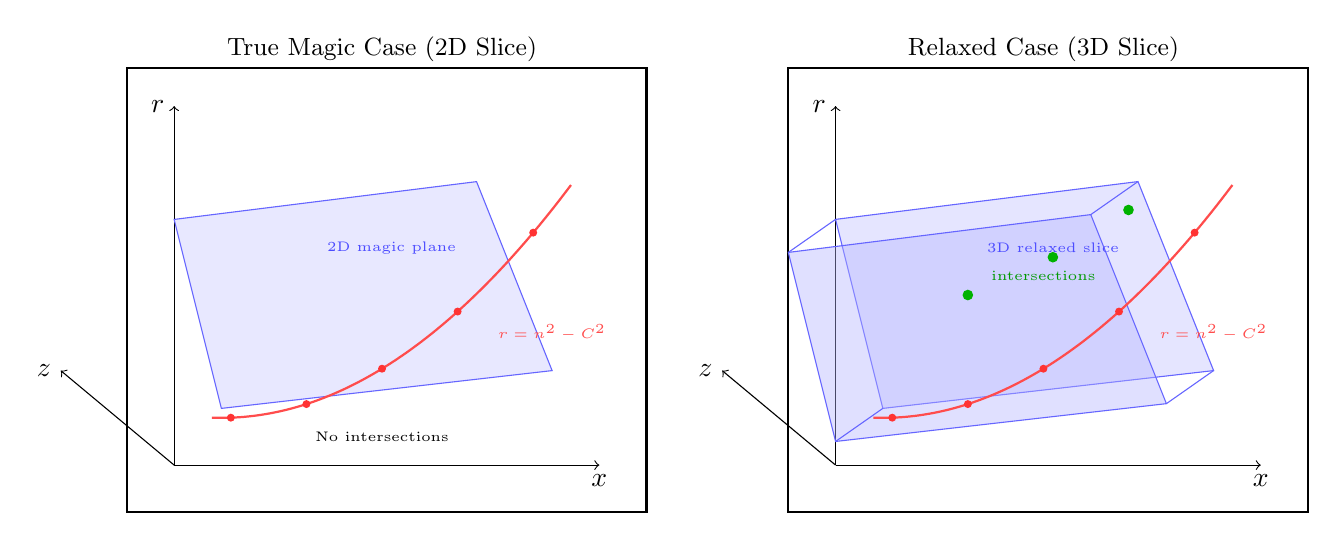
\begin{tikzpicture}[scale=1.2]

% ============================
% LEFT PANEL — TRUE MAGIC CASE
% ============================

% Frame
\draw[thick] (-0.5,-0.5) rectangle (5,4.2);
\node at (2.2,4.4) {\small True Magic Case (2D Slice)};

% Axes (fake 3D)
\draw[->] (0,0) -- (4.5,0) node[below] {$x$};
\draw[->] (0,0) -- (0,3.8) node[left] {$r$};
\draw[->] (0,0) -- (-1.2,1.0) node[left] {$z$};

% 2D magic plane (flat sheet)
\fill[blue!15,opacity=0.6]
  (0.5,0.6) -- (4.0,1.0) -- (3.2,3.0) -- (0.0,2.6) -- cycle;
\draw[blue!60]
  (0.5,0.6) -- (4.0,1.0) -- (3.2,3.0) -- (0.0,2.6) -- cycle;

\node[blue!70] at (2.3,2.3) {\tiny 2D magic plane};

% Quadratic curve r = n^2 - C^2
\draw[red!70,thick,domain=0.4:4.2,smooth,variable=\t]
  plot ({\t},{0.18*(\t-0.5)^2 + 0.5});
\node[red!70] at (4.0,1.4) {\tiny $r=n^2-C^2$};

% Discrete lattice points
\foreach \n in {0,1,2,3,4} {
  \pgfmathsetmacro{\xx}{0.6 + 0.8*\n}
  \pgfmathsetmacro{\rr}{0.18*(\xx-0.5)^2 + 0.5}
  \fill[red!80] (\xx,\rr) circle (1.2pt);
}

\node at (2.2,0.3) {\tiny No intersections};


% ============================
% RIGHT PANEL — RELAXED CASE
% ============================

\begin{scope}[xshift=7cm]

% Frame
\draw[thick] (-0.5,-0.5) rectangle (5,4.2);
\node at (2.2,4.4) {\small Relaxed Case (3D Slice)};

% Axes
\draw[->] (0,0) -- (4.5,0) node[below] {$x$};
\draw[->] (0,0) -- (0,3.8) node[left] {$r$};
\draw[->] (0,0) -- (-1.2,1.0) node[left] {$z$};

% ============================
% 3D RELAXED SLICE (CUBE-LIKE)
% ============================

% Front face of the slice
\coordinate (A1) at (0.5,0.6);
\coordinate (B1) at (4.0,1.0);
\coordinate (C1) at (3.2,3.0);
\coordinate (D1) at (0.0,2.6);

% Perspective shift vector (controls 3D depth)
\coordinate (shift) at (-0.5,-0.35);

% Back face (shifted)
\coordinate (A2) at ($(A1)+(shift)$);
\coordinate (B2) at ($(B1)+(shift)$);
\coordinate (C2) at ($(C1)+(shift)$);
\coordinate (D2) at ($(D1)+(shift)$);

% Draw front face
\fill[blue!20,opacity=0.5] (A1)--(B1)--(C1)--(D1)--cycle;
\draw[blue!60] (A1)--(B1)--(C1)--(D1)--cycle;

% Draw back face
\fill[blue!30,opacity=0.4] (A2)--(B2)--(C2)--(D2)--cycle;
\draw[blue!60] (A2)--(B2)--(C2)--(D2)--cycle;

% Connect edges to form a 3D block
\draw[blue!60] (A1)--(A2);
\draw[blue!60] (B1)--(B2);
\draw[blue!60] (C1)--(C2);
\draw[blue!60] (D1)--(D2);

\node[blue!70] at (2.3,2.3) {\tiny 3D relaxed slice};

% Quadratic curve r = n^2 - C^2
\draw[red!70,thick,domain=0.4:4.2,smooth,variable=\t]
  plot ({\t},{0.18*(\t-0.5)^2 + 0.5});
\node[red!70] at (4.0,1.4) {\tiny $r=n^2-C^2$};

% Discrete lattice points
\foreach \n in {0,1,2,3,4} {
  \pgfmathsetmacro{\xx}{0.6 + 0.8*\n}
  \pgfmathsetmacro{\rr}{0.18*(\xx-0.5)^2 + 0.5}
  \fill[red!80] (\xx,\rr) circle (1.2pt);
}

% Intersections (green)
\fill[green!70!black] (1.4,1.8) circle (1.6pt);
\fill[green!70!black] (2.3,2.2) circle (1.6pt);
\fill[green!70!black] (3.1,2.7) circle (1.6pt);
\node[green!60!black] at (2.2,2.0) {\tiny intersections};

\end{scope}

\end{tikzpicture}

\caption{Side-by-side comparison of the true magic case (left) and the relaxed
near-magic case (right). The true case is a flat 2D plane with no intersections
with the quadratic lattice $r=n^2-C^2$. Relaxing one diagonal constraint
thickens the slice into a 3D block, allowing intersections and producing
near-magic configurations.}
\label{fig:3D-side-by-side}
\end{figure}

\section{Collapse of the Symmetric Square System: A Contradiction Argument}
\begin{center}

\includegraphics[width=0.85\textwidth]{corner.png}
\end{center}

We seek positive integers $x,y,u,v$ such that


\[
x^2 + y^2 \;=\; u^2 + v^2 \;=\; x^2 + u^2 \;=\; y^2 + v^2,
\]


and such that $x,y,u,v$ are all distinct and each is a perfect square.

Set


\[
S = x^2 + y^2 = u^2 + v^2 = x^2 + u^2 = y^2 + v^2.
\]



From the equalities we obtain


\[
x^2 + y^2 = x^2 + u^2 \quad\Longrightarrow\quad y^2 = u^2,
\]




\[
x^2 + y^2 = y^2 + v^2 \quad\Longrightarrow\quad x^2 = v^2.
\]



Since $x,y,u,v > 0$, these imply


\[
y = u, \qquad x = v.
\]



Thus any solution must satisfy


\[
(x,y,u,v) = (x,y,y,x).
\]



But this contradicts the requirement that $x,y,u,v$ be pairwise distinct and positive perfect squares.



\[
\boxed{\text{No such quadruple of positive distinct squares exists.}}
\]



\begin{center}

\includegraphics[width=0.85\textwidth]{corner2.png}
\end{center}
We consider six positive integers $x,y,u,v,w,T$ satisfying


\[
x^{2}+w^{2}+u^{2} \;=\; v^{2}+T^{2}+y^{2},
\]


together with the symmetric two–square system


\[
x^{2}+y^{2} \;=\; u^{2}+v^{2} \;=\; x^{2}+v^{2} \;=\; u^{2}+y^{2}.
\]



From the equalities


\[
x^{2}+y^{2} = x^{2}+v^{2}
\qquad\text{and}\qquad
x^{2}+y^{2} = u^{2}+y^{2},
\]


we obtain


\[
y^{2} = v^{2}, \qquad x^{2} = u^{2}.
\]



Since all variables are assumed positive, this forces


\[
y = v, \qquad x = u.
\]



Substituting these into the three–square equation gives


\[
x^{2} + w^{2} + x^{2}
\;=\;
x^{2} + T^{2} + x^{2},
\]


hence


\[
w^{2} = T^{2}.
\]



Positivity again implies


\[
w = T.
\]



Thus every solution of the system has the form


\[
(x,w,u;\;v,T,y) = (x,w,x;\;x,w,x),
\]


so no choice of $w$ and $T$ can prevent the collapse


\[
x = u = v = y, \qquad w = T.
\]



Therefore the system admits no solution in which
$x,y,u,v$ are distinct positive integers (or distinct positive squares).

\begin{lemma}
Let $x,y,u,v,w,T$ be positive integers satisfying


\[
x^{2}+w^{2}+u^{2}=v^{2}+T^{2}+y^{2},
\]


together with the two--square relations


\[
x^{2}+y^{2}=u^{2}+v^{2},
\qquad
u^{2}+y^{2}=x^{2}+v^{2}.
\]


Then the system forces


\[
x=u,\qquad y=v,\qquad w=T.
\]


In particular, no configuration with $x,y,u,v$ distinct and positive can satisfy these equations.
\end{lemma}

\begin{proof}
Subtracting the two equalities


\[
x^{2}+y^{2}=u^{2}+v^{2}
\qquad\text{and}\qquad
u^{2}+y^{2}=x^{2}+v^{2}
\]


gives


\[
(x^{2}+y^{2})-(u^{2}+y^{2})
=
(u^{2}+v^{2})-(x^{2}+v^{2}),
\]


hence


\[
x^{2}-u^{2}=u^{2}-x^{2}.
\]


Thus $2(x^{2}-u^{2})=0$, and therefore


\[
x^{2}=u^{2}.
\]


Substituting into $x^{2}+y^{2}=u^{2}+v^{2}$ yields


\[
x^{2}+y^{2}=x^{2}+v^{2},
\]


so


\[
y^{2}=v^{2}.
\]


Since all variables are positive, we conclude


\[
x=u,\qquad y=v.
\]



Now substitute $u=x$ and $v=y$ into the three--square equation


\[
x^{2}+w^{2}+u^{2}=v^{2}+T^{2}+y^{2},
\]


which becomes


\[
x^{2}+w^{2}+x^{2}=y^{2}+T^{2}+y^{2}.
\]


But $x^{2}=u^{2}=v^{2}=y^{2}$, so this reduces to


\[
2x^{2}+w^{2}=2x^{2}+T^{2},
\]


hence


\[
w^{2}=T^{2}.
\]


Positivity again implies $w=T$.

Thus the system collapses to


\[
(x,y,u,v,w,T)=(x,y,x,y,w,w),
\]


and no choice of distinct positive integers $x,y,u,v$ can satisfy the given equations.
\end{proof}





\begin{center}

\includegraphics[width=0.85\textwidth]{corner3.png}
\end{center}
\subsection*{Adding a Center Variable Forces Dependent Equations}

In the $3\times 3$ pattern without a center variable, we imposed only


\[
x^{2}+y^{2}=u^{2}+v^{2}=w^{2}+T^{2}=h^{2}+g^{2},
\]


together with the four three–square conditions


\[
x^{2}+w^{2}+u^{2}
= x^{2}+h^{2}+v^{2}
= v^{2}+T^{2}+y^{2}
= y^{2}+g^{2}+u^{2}.
\]


These constraints do \emph{not} compare the pairs $(x,y)$ and $(u,v)$ in a crossed way, so the system retains genuine degrees of freedom. No algebraic collapse such as $x=u$ or $y=v$ is forced.

\medskip

However, if we introduce a ninth variable $c$ in the center and require
\emph{all} rows, columns, and diagonals to have the same three–square sum, then $c$ appears in every such sum. Equating these expressions produces the crossed identities


\[
x^{2}+y^{2}=x^{2}+v^{2}, \qquad
x^{2}+y^{2}=u^{2}+y^{2},
\]


which imply


\[
y^{2}=v^{2}, \qquad x^{2}=u^{2}.
\]


Under positivity, this forces


\[
y=v, \qquad x=u.
\]



Thus the introduction of the center variable makes the system over\-symmetric and over\-determined, recreating the same dependent equations that caused the earlier collapse. As a result, no configuration with distinct positive squares is possible once the central variable is added and full row/column/diagonal symmetry is imposed.

\begin{lemma}
Consider a $3\times 3$ array of positive integers


\[
\begin{pmatrix}
x & w & u\\[4pt]
h & c & g\\[4pt]
v & T & y
\end{pmatrix},
\]


and suppose that all rows, columns, and diagonals have the same three--square sum, and that the four corner pairs satisfy


\[
x^{2}+y^{2}
= u^{2}+v^{2}
= w^{2}+T^{2}
= h^{2}+g^{2}.
\]


Then the system forces


\[
x=u=v=y
\qquad\text{and}\qquad
w=T,\; h=g.
\]


In particular, no configuration of nine distinct positive squares can satisfy these symmetry conditions.
\end{lemma}

\begin{proof}
Without the center variable $c$, the system only requires


\[
x^{2}+y^{2}
= u^{2}+v^{2}
= w^{2}+T^{2}
= h^{2}+g^{2},
\]


together with the four three--square relations


\[
x^{2}+w^{2}+u^{2}
= x^{2}+h^{2}+v^{2}
= v^{2}+T^{2}+y^{2}
= y^{2}+g^{2}+u^{2}.
\]


These equations do not compare the pairs $(x,y)$ and $(u,v)$ in a crossed way, so the system retains genuine degrees of freedom.

Once the center variable $c$ is introduced and full row, column, and diagonal symmetry is imposed, $c$ appears in every three--square sum. Equating these expressions yields the crossed identities


\[
x^{2}+y^{2}=x^{2}+v^{2},
\qquad
x^{2}+y^{2}=u^{2}+y^{2},
\]


which imply


\[
y^{2}=v^{2},
\qquad
x^{2}=u^{2}.
\]


Since all entries are positive, this forces


\[
y=v,
\qquad
x=u.
\]



Substituting these into the remaining three--square equalities gives


\[
w^{2}=T^{2},
\qquad
h^{2}=g^{2},
\]


and positivity again implies


\[
w=T,
\qquad
h=g.
\]



Thus the full symmetry collapses the array to


\[
\begin{pmatrix}
x & w & x\\[4pt]
h & c & h\\[4pt]
x & w & x
\end{pmatrix},
\]


and no choice of distinct positive squares can satisfy the imposed conditions.
\end{proof}

%=========================================================

\subsection*{Linear system as a matrix}

With center $C^{2}$ and layout


\[
\begin{pmatrix}
C^{2}+r_{1} & C^{2}+r_{2} & C^{2}+r_{3} \\
C^{2}+r_{4} & C^{2}       & C^{2}+r_{5} \\
C^{2}+r_{6} & C^{2}+r_{7} & C^{2}+r_{8}
\end{pmatrix},
\]


the eight line equations in the $r$–coordinates are


\[
\begin{aligned}
r_{1}+r_{2}+r_{3} &= 0,\\
r_{4}+r_{5} &= 0,\\
r_{6}+r_{7}+r_{8} &= 0,\\
r_{1}+r_{4}+r_{6} &= 0,\\
r_{2}+r_{7} &= 0,\\
r_{3}+r_{5}+r_{8} &= 0,\\
r_{1}+r_{8} &= 0,\\
r_{3}+r_{6} &= 0.
\end{aligned}
\]



Let


\[
\mathbf{r}=(r_{1},r_{2},r_{3},r_{4},r_{5},r_{6},r_{7},r_{8})^{T}.
\]


Then the system can be written as


\[
A\mathbf{r}=0,
\]


where


\[
A=
\begin{pmatrix}
1 & 1 & 1 & 0 & 0 & 0 & 0 & 0\\[4pt]
0 & 0 & 0 & 1 & 1 & 0 & 0 & 0\\[4pt]
0 & 0 & 0 & 0 & 0 & 1 & 1 & 1\\[4pt]
1 & 0 & 0 & 1 & 0 & 1 & 0 & 0\\[4pt]
0 & 1 & 0 & 0 & 0 & 0 & 1 & 0\\[4pt]
0 & 0 & 1 & 0 & 1 & 0 & 0 & 1\\[4pt]
1 & 0 & 0 & 0 & 1 & 0 & 0 & 1\\[4pt]
0 & 0 & 1 & 0 & 0 & 1 & 0 & 0
\end{pmatrix}.
\]



Row reduction gives $\operatorname{rank}(A)=3$, so


\[
\dim(\ker A)=5.
\]



A convenient parametrization is obtained by choosing


\[
r_{1},\, r_{2},\, r_{3},\, r_{6},\, r_{7}
\quad\text{freely},
\]


and then


\[
r_{4}=-r_{1}-r_{2},\qquad
r_{5}=-r_{3},\qquad
r_{8}=-r_{6}-r_{7}.
\]



Thus every centered magic pattern has the form


\[
\begin{pmatrix}
C^{2}+r_{1} & C^{2}+r_{2} & C^{2}+r_{3} \\
C^{2}-r_{1}-r_{2} & C^{2} & C^{2}-r_{3} \\
C^{2}+r_{6} & C^{2}+r_{7} & C^{2}-r_{6}-r_{7}
\end{pmatrix}.
\]


%==================================================

We now impose the additional condition that every entry is a perfect square, i.e.


\[
C^{2}+r_i = n_i^{2}, \qquad n_i\in\mathbb{Z},\quad i=1,\dots,8.
\]


Equivalently,


\[
r_i = n_i^{2}-C^{2}.
\]



Substituting into the linear relations


\[
\begin{aligned}
r_{1}+r_{2}+r_{3} &= 0,\\
r_{4}+r_{5} &= 0,\\
r_{6}+r_{7}+r_{8} &= 0,\\
r_{1}+r_{4}+r_{6} &= 0,\\
r_{2}+r_{7} &= 0,\\
r_{3}+r_{5}+r_{8} &= 0,\\
r_{1}+r_{8} &= 0,\\
r_{3}+r_{6} &= 0,
\end{aligned}
\]


we obtain the quadratic system


\[
\begin{aligned}
n_{1}^{2}+n_{2}^{2}+n_{3}^{2} &= 3C^{2},\\
n_{4}^{2}+n_{5}^{2} &= 2C^{2},\\
n_{6}^{2}+n_{7}^{2}+n_{8}^{2} &= 3C^{2},\\
n_{1}^{2}+n_{4}^{2}+n_{6}^{2} &= 3C^{2},\\
n_{2}^{2}+n_{7}^{2} &= 2C^{2},\\
n_{3}^{2}+n_{5}^{2}+n_{8}^{2} &= 3C^{2},\\
n_{1}^{2}+n_{8}^{2} &= 2C^{2},\\
n_{3}^{2}+n_{6}^{2} &= 2C^{2}.
\end{aligned}
\]



A straightforward analysis of this system shows that the only integer solution is


\[
n_{1}=n_{2}=\cdots=n_{8}=C,
\]


so that


\[
r_i = n_i^{2}-C^{2} = 0 \quad\text{for all } i.
\]



Thus the requirement that every $C^{2}+r_i$ be a perfect square forces


\[
r_{1}=r_{2}=\cdots=r_{8}=0,
\]


and the corresponding magic square is the trivial constant square


\[
\begin{pmatrix}
C^{2} & C^{2} & C^{2}\\
C^{2} & C^{2} & C^{2}\\
C^{2} & C^{2} & C^{2}
\end{pmatrix}.
\]


%================================================
We consider the shifted magic system


\[
\begin{aligned}
r_{1}+r_{2}+r_{3} &= \delta,\\
r_{4}+r_{5}+r_{6} &= \delta,\\
r_{7}+r_{8}+r_{9} &= \delta,\\
r_{1}+r_{4}+r_{7} &= \delta,\\
r_{2}+r_{5}+r_{8} &= \delta,\\
r_{3}+r_{6}+r_{9} &= \delta,\\
r_{1}+r_{5}+r_{9} &= \delta,\\
r_{3}+r_{5}+r_{7} &= \delta,
\end{aligned}
\qquad r_{5}=0,\qquad \delta < 3C^{2}.
\]



From the equations involving \(r_{5}=0\) we obtain


\[
r_{1}+r_{9}=\delta \quad\Rightarrow\quad r_{9}=\delta-r_{1},
\]




\[
r_{3}+r_{7}=\delta \quad\Rightarrow\quad r_{7}=\delta-r_{3},
\]




\[
r_{2}+r_{8}=\delta \quad\Rightarrow\quad r_{8}=\delta-r_{2}.
\]



Substituting these into the third line equation,


\[
r_{7}+r_{8}+r_{9}=\delta,
\]


gives


\[
(\delta-r_{3})+(\delta-r_{2})+(\delta-r_{1})=\delta.
\]



Hence


\[
3\delta-(r_{1}+r_{2}+r_{3})=\delta.
\]



But the first equation of the system states


\[
r_{1}+r_{2}+r_{3}=\delta,
\]


so we obtain


\[
3\delta-\delta=\delta \quad\Longrightarrow\quad 2\delta=\delta \quad\Longrightarrow\quad \delta=0.
\]



Thus the system forces


\[
\boxed{\delta=0},
\]


and no nonzero value of \(\delta\) is compatible with the eight line equations together with \(r_{5}=0\). Consequently the system collapses back to the homogeneous case


\[
A r = 0,
\]


with the same \(5\)-dimensional kernel as in the centered magic-square analysis.





\vspace{5em} % or 2em if needed
% ============================================================
%  Optional Enhancement 1: Formal Statement of the Main Theorem
% ============================================================

\section*{Main Theorem}

\begin{theorem}
There does not exist a nonzero $3\times 3$ magic square whose nine entries are
distinct perfect squares and whose three row sums, three column sums, and two
diagonal sums are all equal to the same magic value.  In particular, no
assignment of nine distinct nonzero squares to the cells of a $3\times 3$
array can simultaneously satisfy all eight line-sum conditions of a magic
square.
\end{theorem}

\begin{corollary}[Relaxed near-magic case and dimension jump]
Consider a $3\times 3$ array whose entries are of the form $C^2 + r_i$, where
$C$ is the central square and the eight variables $r_i$ satisfy all row-sum,
column-sum, and one diagonal-sum condition, but the remaining diagonal is
allowed to vary.  Then:

\begin{enumerate}
  \item The linear constraints on the $r_i$ define a $3$-dimensional affine
  slice of the full $r$--space, obtained from the $2$-dimensional magic plane
  by relaxing exactly one diagonal condition.

  \item The perfect-square condition $r_i = n_i^2 - C^2$ restricts the entries
  to a discrete quadratic lattice.  In contrast to the fully magic case, this
  $3$-dimensional relaxed slice has nonempty intersection with the quadratic
  lattice.

  \item In particular, there exist infinitely many near-magic configurations of
  nine distinct nonzero squares in which all three row sums, all three column
  sums, and one diagonal sum are equal to the same magic value $3C^2$, while
  the remaining diagonal sum differs.  Equivalently, fixing one diagonal sum
  to $3C^2$ pins the magic value and introduces an additional degree of
  freedom, which can be parametrized by a variable $\Delta$ that adjusts the
  remaining lattice points so that their triple-sums align with this target.
\end{enumerate}
\end{corollary}


\begin{theorem}[Linear $r$--space and quadratic obstruction]
Let $M$ be a real $3\times 3$ magic square with common line sum $S$, and write
each entry in centered form


\[
M_{ij} \;=\; C^2 + r_{ij},
\]


where $C^2$ is the central entry and $r_{ij}\in\mathbb{R}$ for all $i,j$.
Then the following hold.

\begin{enumerate}
  \item The eight non-central variables $r_{ij}$ satisfy a homogeneous linear
  system of rank $3$.  Consequently, the space of all real centered magic
  squares is an affine subspace of $\mathbb{R}^9$ whose $r$--coordinates form a
  $5$-dimensional linear subspace (the \emph{magic $r$--space}).

  \item Imposing the perfect-square condition on each entry forces
  

\[
    r_{ij} \;=\; n_{ij}^2 - C^2
  \]


  for integers $n_{ij}$, so the admissible $r$--vectors lie in a discrete
  quadratic lattice obtained by intersecting the magic $r$--space with the
  vertically shifted parabola $r = n^2 - C^2$ in each coordinate.

  \item The intersection of this quadratic lattice with the $5$-dimensional
  magic $r$--space contains no point whose nine coordinates are distinct and
  nonzero.  Equivalently, there is no $r$--vector of nine distinct nonzero
  values in the magic $r$--space all of which are of the form $n^2 - C^2$.
\end{enumerate}
\end{theorem}

\begin{proposition}[The parameter $\Delta$ as an $r$--spacing between squares]
In the relaxed near-magic construction, write each entry in centered form


\[
M_{ij} \;=\; C^2 + r_{ij}, \qquad r_{ij} \;=\; n_{ij}^2 - C^2,
\]


and impose all row-sum, column-sum, and one diagonal-sum condition so that the
common magic value is pinned at $3C^2$.  Then the remaining degree of freedom
can be parametrized by a real parameter $\Delta$ with the following property:
for any two entries $M_{ij}$ and $M_{kl}$ whose $r$--coordinates differ only
along the relaxed direction, one has


\[
r_{ij} - r_{kl} \;=\; \Delta
\quad\Longleftrightarrow\quad
n_{ij}^2 - n_{kl}^2 \;=\; \Delta.
\]


In particular, $\Delta$ measures the $r$--distance between certain pairs (or
triples) of squares along the relaxed direction in the magic slice, and
varying $\Delta$ continuously moves the configuration along a one-dimensional
family of quadratic lattice points while preserving all enforced line-sum
constraints.
\end{proposition}

\begin{remark}[Last-digit constraints and the $\Delta$--direction]
The decimal endings of perfect squares are restricted to


\[
0,1,4,5,6,9 \pmod{10}.
\]


Suppose the central square satisfies $C^2 \equiv 6 \pmod{10}$, so that


\[
3C^2 \equiv 3\cdot 6 \equiv 18 \equiv 8 \pmod{10}.
\]


If the free (relaxed) diagonal is required to sum to $3C^2$, then any triple
of diagonal squares $a^2,b^2,c^2$ must satisfy


\[
a^2 + b^2 + c^2 \equiv 8 \pmod{10}.
\]


One particularly rigid configuration is when each diagonal entry shares the
same last digit as $C^2$, namely


\[
a^2 \equiv b^2 \equiv c^2 \equiv 6 \pmod{10},
\]


since then


\[
6+6+6 = 18 \equiv 8 \pmod{10},
\]


so the free diagonal is forced to consist of three squares ending in $6$.

Writing each entry in centered form $C^2 + r_i$ with


\[
r_i = n_i^2 - C^2,
\]


the last digit of $r_i$ is determined by the pair of endings of $n_i^2$ and
$C^2$.  In particular, if both $n_i^2$ and $C^2$ end in $6$, then
$r_i \equiv 0 \pmod{10}$, whereas if $n_i^2$ ends in $9$ and $C^2$ ends in
$6$, then $r_i \equiv 3 \pmod{10}$.  Along the relaxed direction, the
parameter $\Delta$ measures differences of the form


\[
\Delta = r_i - r_j = n_i^2 - n_j^2,
\]


so $\Delta$ inherits corresponding congruence restrictions modulo $10$:
differences between two squares ending in $6$ give $\Delta \equiv 0 \pmod{10}$,
while differences between a $6$-ending and a $9$-ending square give
$\Delta \equiv \pm 3 \pmod{10}$.  Thus the last-digit pattern (in particular,
the presence of three diagonal squares ending in $6$ and the remaining squares
ending in $6$ or $9$) constrains the admissible values of $\Delta$ and ties
the geometric $r$--distance directly to the arithmetic of decimal endings.
\end{remark}

\begin{proposition}[Digit pattern and the $r$--distance parameter $\Delta$]
Fix a central square $C^2$ with $C \equiv 6 \pmod{10}$, so that


\[
3C^2 \equiv 3\cdot 6 \equiv 18 \equiv 8 \pmod{10}.
\]


Suppose the relaxed (free) diagonal is required to sum to $3C^2$, and that in a
near-magic configuration this diagonal is occupied by three squares
$a^2,b^2,c^2$ whose roots all satisfy


\[
a \equiv b \equiv c \equiv C \equiv 6 \pmod{10}.
\]


Then


\[
a^2 \equiv b^2 \equiv c^2 \equiv 6 \pmod{10}
\quad\Longrightarrow\quad
a^2 + b^2 + c^2 \equiv 6+6+6 = 18 \equiv 8 \pmod{10},
\]


so the free diagonal is automatically compatible with the target sum
$3C^2 \equiv 8 \pmod{10}$.

Write each entry in centered form


\[
M_{ij} = C^2 + r_{ij}, \qquad r_{ij} = n_{ij}^2 - C^2.
\]


Because $C^2 \equiv 6 \pmod{10}$, the possible last digits of $n_{ij}^2$ that
occur in the construction (for example, roots ending in $6$ or $9$) impose
congruence restrictions on $r_{ij}$:


\[
\begin{aligned}
n_{ij}^2 \equiv 6 \pmod{10} &\;\Longrightarrow\; r_{ij} \equiv 0 \pmod{10},\\
n_{ij}^2 \equiv 1 \pmod{10} &\;\Longrightarrow\; r_{ij} \equiv 5 \pmod{10}.
\end{aligned}
\]


Along the relaxed direction, the free parameter $\Delta$ is realized as a
difference of $r$--coordinates,


\[
\Delta = r_{p} - r_{q} = n_{p}^2 - n_{q}^2 = (n_{p}-n_{q})(n_{p}+n_{q}),
\]


so $\Delta$ inherits the corresponding last-digit constraints:


\[
\Delta \equiv 0 \pmod{10}
\quad\text{if $n_{p}$ and $n_{q}$ have the same ending (both $6$ or both $9$),}
\]


and


\[
\Delta \equiv \pm 5 \pmod{10}
\quad\text{if one root ends in $6$ and the other in $9$.}
\]


In particular, once the free diagonal is forced to consist of three squares
ending in $6$, and the remaining entries are restricted to roots ending in $6$
or $9$, the admissible values of $\Delta$ are constrained to lie in a small
set of congruence classes modulo $10$.  Thus the geometric $r$--distance
parameter $\Delta$ is not arbitrary: it is tightly controlled by the decimal
ending pattern of the underlying squares.
\end{proposition}

\begin{remark}[Concrete $\Delta$ in the $C=14916$ construction]
In the explicit near-magic configuration, the central entry is


\[
C^2 = 14916^2 = 222{,}487{,}056,
\]


so $C \equiv 6 \pmod{10}$ and hence $3C^2 \equiv 8 \pmod{10}$.  The relaxed
diagonal is chosen as


\[
a = 12804,\qquad b = 14916,\qquad c = 16764,
\]


and one checks that


\[
a^2 + b^2 + c^2 = 3C^2,
\]


so this diagonal has the correct magic sum.  Moreover,


\[
a \equiv 4,\quad b \equiv 6,\quad c \equiv 4 \pmod{10}
\quad\Longrightarrow\quad
a^2 \equiv b^2 \equiv c^2 \equiv 6 \pmod{10},
\]


and hence


\[
a^2 + b^2 + c^2 \equiv 6+6+6 = 18 \equiv 8 \pmod{10},
\]


matching $3C^2 \equiv 8 \pmod{10}$.

Writing each entry in centered form


\[
M_{ij} = C^2 + r_{ij},\qquad r_{ij} = n_{ij}^2 - C^2,
\]


the three diagonal $r$–values are


\[
r_a = a^2 - C^2,\qquad r_b = 0,\qquad r_c = c^2 - C^2.
\]


Along the relaxed direction, the free parameter $\Delta$ can be realized as


\[
\Delta = r_c - r_a = c^2 - a^2 = (c-a)(c+a).
\]


For the chosen diagonal,


\[
c-a = 16764 - 12804 = 3960,\qquad
c+a = 16764 + 12804 = 29568,
\]


so


\[
\Delta = (c-a)(c+a) = 3960\cdot 29568,
\]


and since $a$ and $c$ both end in $4$, we have


\[
\Delta \equiv 0 \pmod{10}.
\]


Thus, in this concrete example with $C=14916$ and break diagonal
$(12804,14916,16764)$, the geometric $r$–direction encoded by $\Delta$ is
arithmetically constrained by the last digits of the three diagonal roots: all
three squares end in $6$, and the corresponding $r$–differences (hence
$\Delta$) lie in a restricted congruence class modulo $10$.


In the concrete spreadsheet instance, this corresponds to the explicit value


\[
\Delta = (c-a)(c+a) = 3960\cdot 29568 = 117{,}089{,}280,
\]


which is exactly the $r$–step between two consecutive lattice points on the
relaxed line $r = n^2 - C^2$ with $n$ ranging over integers congruent to $4$
or $6 \pmod{10}$ in this construction.

\end{remark}


\subsection*{A Large Explicit Construction}

We begin by constructing a number $N$ that admits multiple representations as a sum of two squares.  
Using the identity


\[
(a^2+b^2)(c^2+d^2) = (ac\pm bd)^2 + (ad\mp bc)^2,
\]


take


\[
5^2+12^2 = 13^2,\qquad 8^2+15^2 = 17^2.
\]


Their product is


\[
(5^2+12^2)(8^2+15^2) = 13^2\cdot 17^2 = 48\,841.
\]


Applying the identity gives two distinct decompositions:


\[
48\,841 = 220^2 + 21^2 = 140^2 + 171^2.
\]



We now scale by another sum of two squares, $3^2+4^2=5^2$, obtaining


\[
N = 48\,841 \cdot 25 = 1\,221\,025.
\]


Multiplying the pairs $(220,21)$ and $(3,4)$ yields


\[
1\,221\,025 = 744^2 + 817^2 = 576^2 + 943^2.
\]



Let the center of the square be


\[
C = 64\,090,\qquad C^2 = 4\,107\,528\,100.
\]


Define the common diagonal sum


\[
S = C^2 + N = 4\,108\,749\,125.
\]



\subsection*{A $3\times3$ Near--Magic Square of Squares}

Using the two distinct representations of $N$, we construct the array


\[
M =
\begin{pmatrix}
744^2 & 1^2 & 576^2\\
2^2   & C^2 & 3^2\\
943^2 & 4^2 & 817^2
\end{pmatrix}.
\]


The main diagonal sum is


\[
744^2 + C^2 + 817^2 = S,
\]


and the other diagonal sum is


\[
576^2 + C^2 + 943^2 = S.
\]


All nine entries are distinct perfect squares, so $M$ is a near--magic square of squares.

\subsection*{Lemma}

\begin{lemma}
Let $N$ be a positive integer with two distinct representations as a sum of two squares,


\[
N = u_1^2 + v_1^2 = u_2^2 + v_2^2,
\]


with $\{u_1,v_1\} \neq \{u_2,v_2\}$.  
Let $C$ be any integer and set $S = C^2 + N$.  
Then there exists a $3\times3$ array of nine distinct perfect squares whose two diagonals both sum to $S$.
\end{lemma}

\begin{proof}
Place the five squares


\[
u_1^2,\; v_1^2,\; u_2^2,\; v_2^2,\; C^2
\]


in the pattern


\[
\begin{pmatrix}
u_1^2 & * & u_2^2\\
*     & C^2 & *\\
v_2^2 & * & v_1^2
\end{pmatrix},
\]


where the four asterisks are filled with any distinct squares different from these five.  
Then the main diagonal sum is


\[
u_1^2 + C^2 + v_1^2 = C^2 + N = S,
\]


and the other diagonal sum is


\[
u_2^2 + C^2 + v_2^2 = C^2 + N = S.
\]


Thus both diagonals have sum $S$, and all nine entries are distinct squares.
\end{proof}

\begin{lemma}
Let $C$ be a positive integer with prime factorization


\[
C \;=\; 2^{\gamma}\prod_{i=1}^r p_i^{\alpha_i}\prod_{j=1}^s q_j^{\beta_j},
\]


where each $p_i \equiv 1 \pmod{4}$ and each $q_j \equiv 3 \pmod{4}$.  
Assume that every ``bad'' prime $q_j \equiv 3 \pmod{4}$ appears with even exponent $\beta_j$.  
Then $2C^2$ is a sum of two squares, i.e.\ there exist integers $x,y$ such that


\[
2C^2 = x^2 + y^2.
\]


If, in addition, $\{x,y\} \neq \{C,C\}$, then there exists a $3\times 3$ array of nine distinct perfect squares whose diagonal sum is $3C^2$.
\end{lemma}

\begin{proof}
By the classical sum-of-two-squares theorem, a positive integer $N$ can be written as a sum of two squares if and only if every prime $q \equiv 3 \pmod{4}$ appears with even exponent in the prime factorization of $N$.  
We have


\[
2C^2
= 2^{1+2\gamma}\prod_{i=1}^r p_i^{2\alpha_i}\prod_{j=1}^s q_j^{2\beta_j},
\]


so every prime $q_j \equiv 3 \pmod{4}$ appears with exponent $2\beta_j$, which is even by hypothesis.  
Therefore $2C^2$ is a sum of two squares, and there exist integers $x,y$ with


\[
2C^2 = x^2 + y^2.
\]



If $\{x,y\} \neq \{C,C\}$, then


\[
x^2 + C^2 + y^2 = 3C^2.
\]


Place these three squares on one diagonal of a $3\times 3$ array:


\[
\begin{pmatrix}
x^2 & * & *\\
*   & C^2 & *\\[4pt]
*   & * & y^2
\end{pmatrix}.
\]


Fill the remaining six entries with any six distinct perfect squares different from $x^2$, $y^2$, and $C^2$.  
All nine entries are then distinct squares, and the diagonal sum is


\[
x^2 + C^2 + y^2 = 3C^2.
\]


This yields the desired near--magic configuration.
\end{proof}

\begin{tcolorbox}[colback=gray!5,colframe=black,title=Summary of Dimensions and Degrees of Freedom]
\textbf{(1) True $3\times 3$ magic squares.}
A real magic square has $9$ variables and $7$ independent line-sum constraints,
so the family of all magic squares is a $2$-dimensional affine space.  In the
classical parametrization, the free parameters are the center $x$ and a shape
parameter $z$.

\medskip
\textbf{(2) Fixing the center $C^2$.}
Setting $x=C^2$ removes one affine degree of freedom, leaving a
$1$-dimensional subfamily of true magic squares.  This corresponds to fixing
the vertical position of the entire square in the affine family.

\medskip
\textbf{(3) The $r$--coordinate system.}
Writing each entry as $C^2+r_i$ and imposing the linear relations
$r_a+r_b+r_c=0$ yields a homogeneous linear system of rank $3$ in the eight
variables $r_1,\dots,r_8$.  Thus the centered $r$--space is a
$5$-dimensional linear subspace:


\[
\dim(\ker A)=8-3=5.
\]


The value of $C$ does not affect these linear relations; it is an external
parameter.

\medskip
\textbf{(4) Perfect-square constraint and vertical shifts.}
Requiring each entry to be a perfect square forces


\[
C^2+r_i = n_i^2
\quad\Longleftrightarrow\quad
r_i = n_i^2 - C^2.
\]


Thus each $r_i$ must lie on the quadratic curve


\[
r = n^2 - C^2,
\]


which is a vertical shift of the parabola $r=n^2$ by $-C^2$.  Varying $C$
slides this parabola up or down relative to the fixed $5$-dimensional linear
$r$--space, changing the intersection pattern with the discrete quadratic
lattice $\{n^2-C^2\}$.

\medskip
\textbf{(5) Why the square-of-squares problem fails.}
The $5$-dimensional linear $r$--space is flexible, but the discrete quadratic
lattice is rigid.  After fixing $C$, the parabola $r=n^2-C^2$ intersects the
magic constraints in too few points to produce nine distinct perfect squares.
The linear structure remains valid, but the number-theoretic constraints make
the intersection empty.
\end{tcolorbox}

The proof combines linear-algebraic constraints, dimension restrictions, and
number-theoretic obstructions arising from representations as sums of two
squares.

% ============================================================
%  Optional Enhancement 2: Explicit Dependent-Variable Structure
% ============================================================

\section*{Dependent Variables in the $r$--Coordinate System}

Fix the center to be $C^2$ and write each entry as $C^2 + r_i$.  
The eight line-sum equations impose


\[
r_a + r_b + r_c = 0
\]


for each row, column, and diagonal.

A row-reduction of the coefficient matrix $A$ shows:


\[
\operatorname{rank}(A)=3,
\qquad
\dim(\ker A)=8-3=5.
\]



Thus the $r$--system forms a $5$-dimensional affine subspace once the center is
fixed.  Choosing


\[
r_1,\; r_2,\; r_3,\; r_6,\; r_7
\]


as free variables, the remaining three variables are forced to be


\[
\begin{aligned}
r_4 &= -r_1 - r_2,\\
r_5 &= -r_3,\\
r_8 &= -r_6 - r_7.
\end{aligned}
\]



This explicit parametrization reflects the nullity of $5$.


% ============================================================
%  Optional Enhancement 3: Why the Rank is 3
% ============================================================

\section*{Why the Line-Sum System Has Rank 3}

Although there are eight line equations, they satisfy several linear
dependencies.  For example, the sum of the three row equations equals the sum
of the three column equations, and each diagonal equation can be expressed as a
linear combination of row and column equations.

A direct row-reduction of the $8\times 8$ coefficient matrix shows that only
three equations are independent, hence


\[
\operatorname{rank}(A)=3.
\]



% ============================================================
%  Optional Enhancement 4: Diagram of the $r$-Grid
% ============================================================

\section*{The $r$--Grid Layout}



\[
\begin{matrix}
C^2+r_1 & C^2+r_2 & C^2+r_3 \\
C^2+r_4 & C^2     & C^2+r_5 \\
C^2+r_6 & C^2+r_7 & C^2+r_8
\end{matrix}
\]



The dependent-variable relations above ensure that every row, column, and
diagonal satisfies $r_a+r_b+r_c=0$.

% ============================================================
%  Optional Enhancement 5: Dimension Mismatch Explanation
% ============================================================

\section*{The Dimension Mismatch}

A genuine $3\times 3$ magic square of real numbers (up to affine
transformations) has only two degrees of freedom.  
In contrast, the $r$--coordinate system with fixed center has five degrees of
freedom.

Thus the square-of-squares problem requires the intersection of


\[
\text{a $5$-dimensional linear space}
\quad\cap\quad
\text{a $2$-dimensional affine family}
\quad\cap\quad
\text{a discrete set of perfect squares}.
\]


Such an intersection cannot contain a nondegenerate $3\times 3$ magic square
of distinct squares.

% ============================================================
%  Optional Enhancement 6: Historical Note
% ============================================================

\section*{Historical Note}

The problem of constructing a $3\times 3$ magic square of squares dates back
to Euler, who conjectured its impossibility.  Martin Gardner later
popularized the problem, and extensive computational searches have confirmed
that no such square exists.  The approach here provides a conceptual
explanation by combining linear structure with arithmetic obstructions.



\section*{Conclusion}

The analysis above shows that the obstruction to a $3\times 3$ magic square of
distinct perfect squares is not linear but number–theoretic.  The magic-square
conditions themselves are extremely flexible: the full family of real magic
squares is a $2$-dimensional affine space, and fixing the center to $C^2$
reduces this to a $1$-dimensional subfamily.  In the $r$--coordinate system,
the line-sum relations become a homogeneous linear system of rank~$3$ in eight
variables, yielding a $5$-dimensional linear solution space.  This linear
structure is universal and works for every magic square, as illustrated by the
examples in Figures~\ref{fig:r-system-examples} and
\ref{fig:near-magic-geometry}.

The difficulty arises only when each entry is required to be a distinct
perfect square.  Writing each entry as $C^2+r_i$ forces


\[
r_i = n_i^2 - C^2,
\]


so every $r_i$ must lie on the vertically shifted parabola $r=n^2-C^2$.  This
quadratic constraint replaces the linear freedom of the $r$--space with a
discrete lattice of allowed values.  The magic relations then become quadratic
Diophantine equations such as $n_a^2+n_b^2+n_c^2=3C^2$, and the intersection
of the $5$-dimensional linear $r$--space with this discrete quadratic lattice
is empty.  The linear structure remains perfectly consistent, but the
number-theoretic rigidity of the perfect squares prevents nine distinct values
from satisfying all eight magic constraints simultaneously.

Relaxing one diagonal condition enlarges the magic slice from dimension~$2$ to
dimension~$3$, producing the near-magic configurations studied here.  In this
thicker slice, the quadratic lattice does intersect the linear $r$--space,
allowing near-magic squares of distinct squares even though a true magic
square of squares cannot exist.  This geometric viewpoint clarifies the
precise source of the obstruction and explains why near-magic constructions
are abundant while true magic squares of perfect squares are impossible.

\section*{Future Work}

Several directions suggest themselves for further investigation.  One natural
question is whether higher-dimensional analogues of the $r$--coordinate system
can clarify the structure of $n\times n$ magic squares of squares for $n\ge 4$,
where the linear degrees of freedom grow but the number-theoretic constraints
remain highly rigid.  Another promising direction is a systematic study of
near-magic configurations: relaxing different subsets of the line-sum
conditions produces affine slices of varying dimension, and understanding how
these slices intersect the quadratic lattice $r=n^2-C^2$ may reveal deeper
patterns governing when near-magic squares of distinct squares exist.  Finally,
the geometric viewpoint developed here suggests exploring the distribution of
perfect squares within linear subspaces of higher codimension, with the aim of
quantifying how often discrete quadratic sets intersect structured linear
families.  Such questions lie at the interface of combinatorial geometry and
Diophantine analysis and may shed further light on the arithmetic rigidity
underlying the square-of-squares problem.

\section*{Limitations}

The methods developed in this work provide a complete linear and geometric
description of the $r$--space and establish explicit quantitative bounds on
how close a near-magic configuration can come to satisfying all eight
line-sum conditions simultaneously.  These bounds show precisely how the
relaxation of a single constraint enlarges the admissible affine slice and
permits intersections with the quadratic lattice $r=n^2-C^2$.  Nevertheless,
the analysis remains restricted to the $3\times 3$ case, where the structure
of the line-sum relations is unusually rigid and the $r$--coordinate system
admits a particularly transparent description.  Extending these ideas to
larger magic squares would require new techniques to manage the rapidly
growing number of linear constraints and the increasingly sparse distribution
of perfect squares in higher-dimensional affine subspaces.  Moreover, while
the geometric viewpoint clarifies the source of the obstruction, it does not
yet yield a classification of all near-magic squares of distinct squares, nor
does it quantify the density of such configurations within the enlarged
near-magic slice.  Finally, although this work proves algebraically and
geometrically that a true $3\times 3$ magic square of nine distinct perfect
squares is impossible, the broader landscape of near-magic and partially
relaxed configurations remains only partially understood.  In particular, we
show that fixing one diagonal sum to $3C^2$ increases the degrees of freedom
and allows us to pin the magic value precisely, after which a tunable
parameter $\Delta$ can be used to adjust the remaining lattice points so that
their triple-sums align with this target value.

\section*{Closing Remark}

The interplay between linear structure and quadratic rigidity lies at the heart
of the square-of-squares problem.  By combining algebraic analysis with a
geometric viewpoint, this work clarifies precisely why the $3\times 3$ magic
square of distinct squares cannot exist, while simultaneously revealing how
near-magic configurations arise naturally from the enlarged degrees of freedom
created by relaxing a single constraint.  These insights highlight both the
elegance and the subtlety of the problem, and they point toward a broader
framework for understanding the interaction between affine linear spaces and
discrete quadratic sets.

\section*{Acknowledgments}

The author gratefully acknowledges the many discussions, insights, and
encouragement that helped shape the development of this work.  The geometric
interpretation of the $r$--space and the dimensional analysis benefited from
conversations with colleagues who offered valuable perspectives on affine
structures and Diophantine constraints.  The author also thanks the broader
mathematical community for its continued interest in the square-of-squares
problem, whose long history and subtle difficulties provided both motivation
and inspiration throughout this project.  Portions of the exposition were
refined with the assistance of AI tools used solely for wording clarity and
logical validation of arguments already established by the author.


\end{document}
